\subsection{Likelihood}
\label{sec:pf-likelihood}

The second component of \gls{rbe} is the update step, which involves accounting for the likelihood of the data given the predicted state, $p(\Vobs_k | \Vstate_k)$. In the \pf{}, as discussed in \cref{sec:pf}, updating is performed by reweighting each of the particles based on their likelihoods, $p(\Vobs_k | \Vstate\vi_k)$, and then, if necessary, performing weighted resampling with replacement (importance resampling). That is,
\begin{equation}
\label{eq:vehicle_pf_update}
p(\Vstate_k | \Vobs_{1:k}) \approx
\sum_{i=1}^\Np
    \Pwt_{k}
    \dirac\left(
        \Vstate_k - \Vstate\vi_k
    \right)
\end{equation}
where
\begin{equation}
\label{eq:vehicle_pf_reweight}
\Pwt_k = \frac{
    \Pwt_{k-1} p(\Vobs_k | \Vstate\vi_k)
}{
    \sum_{j=1}^\Np \Pwt[j]_{k-1} p(\Vobs_k | \Vstate\vi[j]_k)
}
\end{equation}


The likelihood function is where the \pf{} is superior in this application. Were we to model the vehicle's state with a \kf{}, we would need to somehow compare a distribution in one dimension (distance travelled) with an observation in two dimensions (\gls{gps} coordinate). \cite{Cathey_2003} used an optimisation technique to obtain an estimated observation of distance travelled based on the observation location, which they then used as data for their \kf{} implementation. However, as demonstrated in \cref{fig:lhood_obs}, there are situations where the ``maximised'' location may be wrong, in which case the resulting state will be eroneous.


The \pf{} effectively checks to see how plausible the observation is assuming each particle is the truth, allowing us to weight each particle by its plausibility. Since there are two types of data, two likelihood functions are required: one for \GPS{} observations, and a second for trip updates. There is no need to match the observations to distance: instead, each particle's state can be transformed into a \gls{gps} coordinate, making it directly compariable to the vehicle's reported location.


\subsubsection{GPS vehicle locations}
\label{sec:lhood_gps}

\begin{knitrout}
\definecolor{shadecolor}{rgb}{0.969, 0.969, 0.969}\color{fgcolor}\begin{figure}
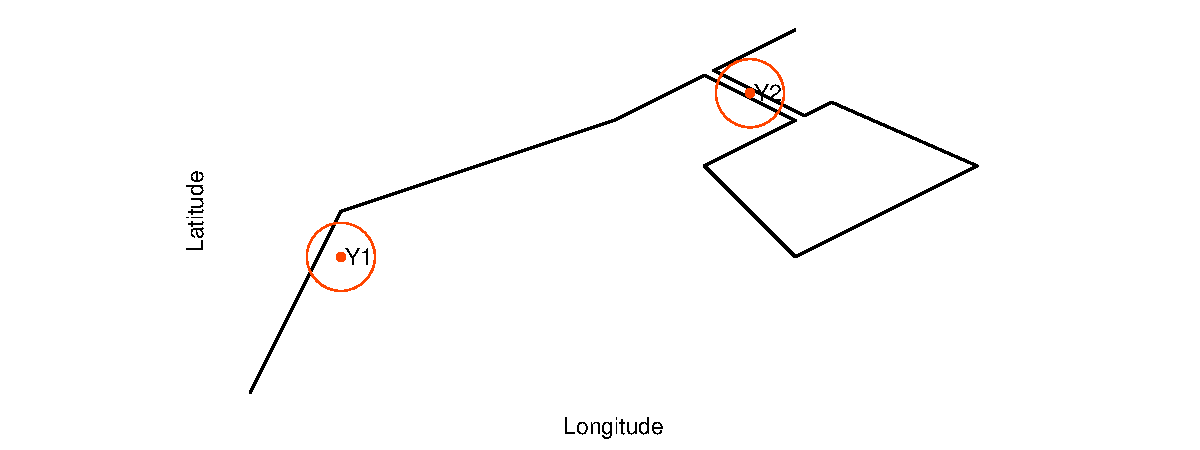
\includegraphics[width=\maxwidth]{figure/lhood_obs-1} \caption[Observations of vehicle on a simple path]{Observations of vehicle on a simple path. The red points indicate the reported GPS positions, with circles indicating the GPS error associated with each observation. Observation Y1 is easy to map to the route, while Y2 is more complicated and has two plausible, distinct locations.}\label{fig:lhood_obs}
\end{figure}


\end{knitrout}





For the \gls{gps} location update, the inherent \gls{gps} error, $\GPSerr$, needs to be filtered out to get better estimates of vehicle state. Examples of positions are shown in \cref{fig:lhood_obs}. A particle's likelihood should represent the geographical \emph{closeness} of the estimated position to the vehicle's reported position. We therefore want the likelihood to depend on the \emph{distance between the observed and predicted} vehicle locations. The first step to computing the likelihood is therefore
to calculate the GPS position of the \emph{particle}, $\Ppos\vi_k$, by using the \emph{measurement function},
\begin{equation}
\label{eq:pf_measurement_fun}
\Ppos\vi_k = \Vmeas(\Vstate\vi_k, \ShapePath)
\end{equation}
which is simply a deterministic function given the route's path, $\ShapePath$, which is a sequence of latitude-longitude pairs and the cumulative distance along the line. Once the geographical position of the particle is obtained, it is compared to the observed vehicle location, as shown in \cref{fig:gps_dist}.

\begin{knitrout}
\definecolor{shadecolor}{rgb}{0.969, 0.969, 0.969}\color{fgcolor}\begin{figure}

{\centering 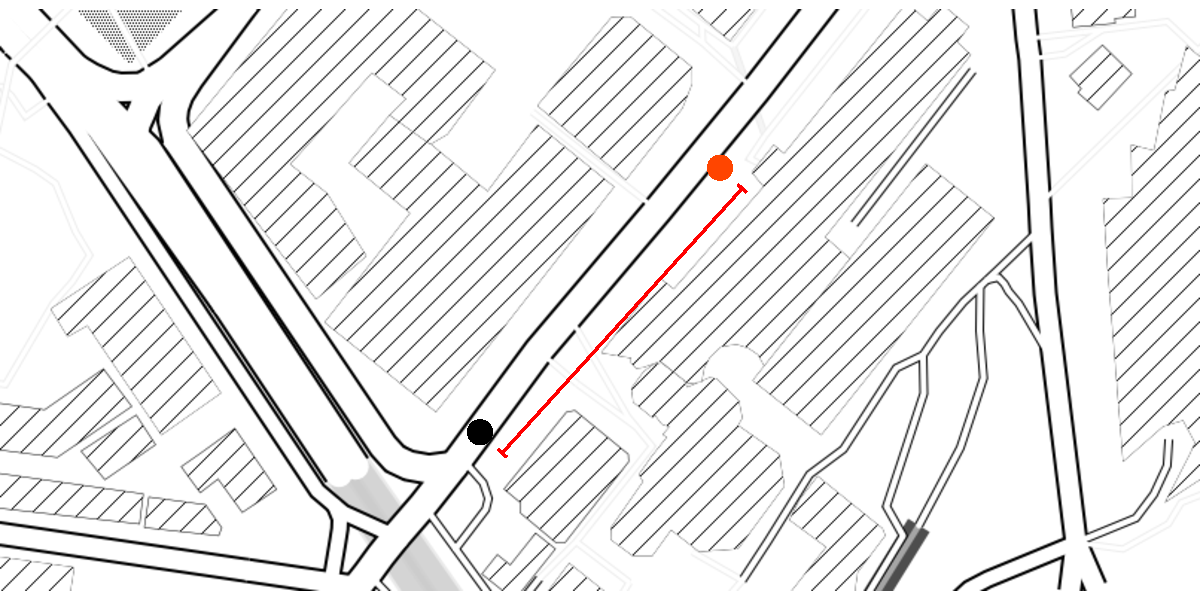
\includegraphics[width=0.8\textwidth]{figure/gps_dist-1} 

}

\caption[GPS distance between two points]{GPS distance between two points. The vehicle's reported location is shown in orange; one particle estimate of it's location is in black. The desired distance is denoted by the red line.}\label{fig:gps_dist}
\end{figure}


\end{knitrout}

Computing the distance between two GPS coordinates can achieved using several formulae, each with varying levels of accuracy. Since all of the distances are going to be (very) small, the \emph{Equirectangular projection} is sufficiently accurate for computing geographical distances \citep{cn}. This projection transforms the point $\Vobs_1 = \tvec{\Vlon_1, \Vlat_1}$, where latitude $\Vlat$ and longitude $\Vlon$ are in radians (the width of one longitudinal radian depends on latitude) onto a surface with meters on both axes, centered on the point $\Vobs_0 = \tvec{\Vlon_0, \Vlat_0}$ and using the Earth's radius $R = 6.371 \times 10^6$m,
\begin{equation}
\label{eq:equirectangular_projection}
\Vproj{\Vobs_1}{\Vobs_0} =
\begin{bmatrix} x \\ y \end{bmatrix} =
R \begin{bmatrix}
(\Vlon_1 - \Vlon_0) \cos \Vlat_0 \\
(\Vlat_1 - \Vlat_0)
\end{bmatrix}
\end{equation}
so that the distance between the points can easily be computed
using their \emph{euclidean distance}
\begin{equation}
\label{eq:obs_dist}
\dist{\Vobs_0, \Vobs_1} = \sqrt{x^2 + y^2}.
\end{equation}
This is shown visually in \cref{fig:gps_projection}.
Note that conversion from degrees to radians is achieved by
multiplying degrees by $\frac{\pi}{180}$.

\begin{knitrout}
\definecolor{shadecolor}{rgb}{0.969, 0.969, 0.969}\color{fgcolor}\begin{figure}

{\centering \subfloat[GPS coordinates\label{fig:gps_projection1}]{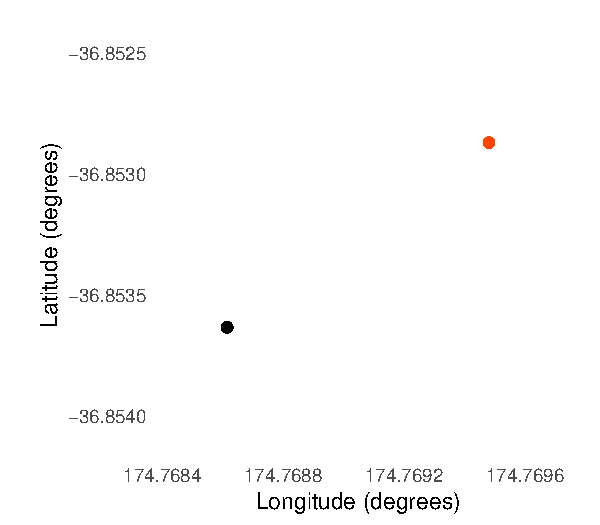
\includegraphics[width=0.49\textwidth]{figure/gps_projection-1} }
\subfloat[Projected points\label{fig:gps_projection2}]{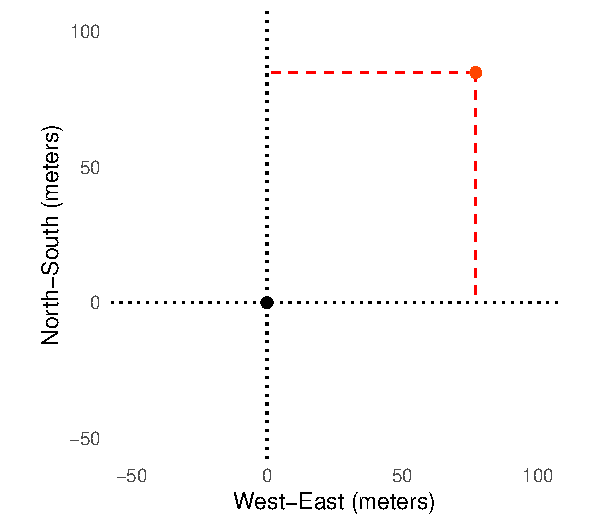
\includegraphics[width=0.49\textwidth]{figure/gps_projection-2} }

}

\caption[Equirectangular projection of GPS coordinates onto flat surface, allowing the distance from each particle to the observed location to easily be calculated]{Equirectangular projection of GPS coordinates onto flat surface, allowing the distance from each particle to the observed location to easily be calculated.}\label{fig:gps_projection}
\end{figure}


\end{knitrout}


Now that spherical observations can be compared on a flat surface,
it is necessary to assume that \GPS{} observations are distributed
as a multivariate random variable around the true position of the vehicle
on the ground,
with a \GPS{} error of $\GPSerr$,
and that the variation does not depend on direction.
That is, if the observation $\Vobs_k$ is projected using
\cref{eq:equirectangular_projection} conditional on the true position
$\Vmeas(\Vstate_k)$,
then the projected point will be a multivariate random variable
$\vec{r}_k \sim \Normal{\vec{0}}{\GPSerr \mat{I}}$.
The above, shown in \cref{fig:gps_error2},
can more simply be expressed by
\begin{equation}
% \label{eq:obs_projection}
\label{eq:gps_error_model}
\Vproj{\Vobs_k}{\Vmeas(\Vstate_k)} =
    \Vproj{\Vmeas(\Vstate_k)}{\Vmeas(\Vstate_k)} + \vec{r}_k
    = \vec{r}_k
\end{equation}

% \begin{equation}
% \Vobs_k = \Viproj{\vec{r}\vi_k}{\Vmeas(\Vstate\vi_k)}.
% \end{equation}

\begin{knitrout}
\definecolor{shadecolor}{rgb}{0.969, 0.969, 0.969}\color{fgcolor}\begin{figure}

{\centering \subfloat[GPS map error\label{fig:gps_error1}]{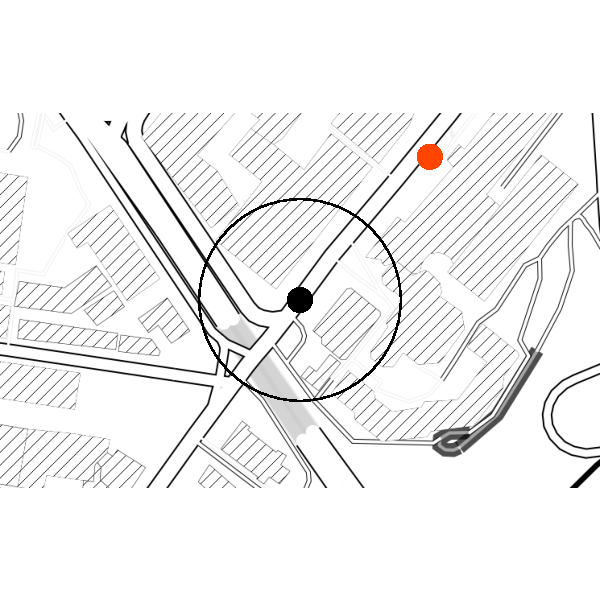
\includegraphics[width=0.49\textwidth]{figure/gps_error-1} }
\subfloat[Projected error\label{fig:gps_error2}]{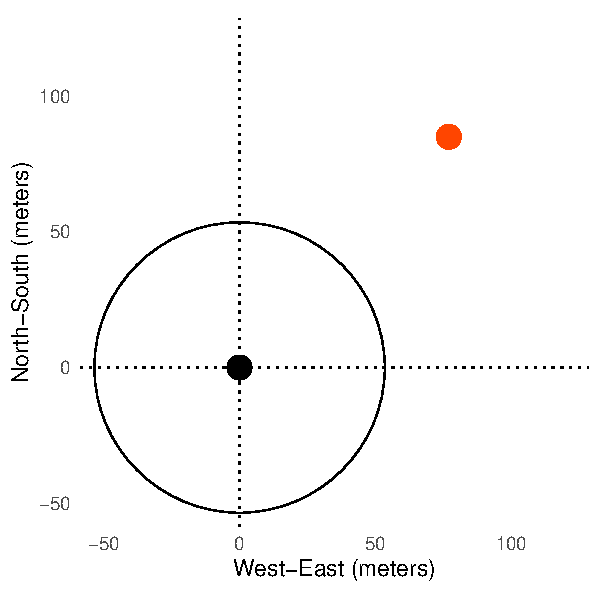
\includegraphics[width=0.49\textwidth]{figure/gps_error-2} }

}

\caption[GPS error is assumed to be circular on a map]{GPS error is assumed to be circular on a map.}\label{fig:gps_error}
\end{figure}


\end{knitrout}


From \cref{eq:equirectangular_projection,eq:obs_dist,eq:gps_error_model}
the distance between the true and observed locations
is the magnitude of the error $\vec{r}_k$,
\begin{equation}
\dist{\Vobs_k, \Vmeas(\Vstate_k)} = ||\vec{r}_k|| =
    \sqrt{r_{k1}^2 + r_{k2}^2}
\end{equation}
However, this error can also be expressed in terms of two independent,
standard normal random variables $z_1, z_2 \sim \Normal{0}{1}$,
such that $r_{jk} = \GPSerrSD z_j$ for $j = 1, 2$,
resulting in
\begin{equation}
\dist{\Vobs_k, \Vmeas(\Vstate\vi_k)} =
    \sqrt{(\GPSerrSD z_1)^2 + (\GPSerrSD z_2)^2} =
    \GPSerrSD \sqrt{z_1^2 + z_2^2}
\end{equation}
Since the distribution of two squared standard normal random variables is known
to be $\chi^2$ distributed with 2~degrees of freedom,
which is itself exponential with rate 0.5
\citep{cn},
then
\begin{equation}
\label{eq:sum_sq_dist}
z_1^2 + z_2^2 \sim \Exp{\frac{1}{2}}
\end{equation}
which, following the [fact] that if $X \sim \Exp{\theta}$,
then $cX \sim \Exp{\frac{\theta}{c}}$,
the squared distance between points is simply represented as
\begin{equation}
\label{eq:distance_distrib}
\dist{\Vobs_k, \Vmeas(\Vstate_k)}^2 \sim \Exp{\frac{1}{2\GPSerr}}
\end{equation}

So now, given a particle state estimate of $\Vstate\vi_k$,
the likelihood of a \GPS{} observation using only
the distance between two coordinates is given by
\begin{equation}
\label{eq:particle_lh_fun}
p(\Vobs_k | \Vstate\vi_k) =
    \frac{1}{2\GPSerr} \exp\left\{
        - \frac{\dist{\Vobs_k, \Vmeas(\Vstate\vi_k)}^2}{2\GPSerr}
    \right\}
\end{equation}
allowing the particles to be reweighted using \cref{eq:vehicle_pf_reweight}.
This is shown visually in \cref{fig:pf_wts}.


\begin{knitrout}
\definecolor{shadecolor}{rgb}{0.969, 0.969, 0.969}\color{fgcolor}\begin{figure}

{\centering 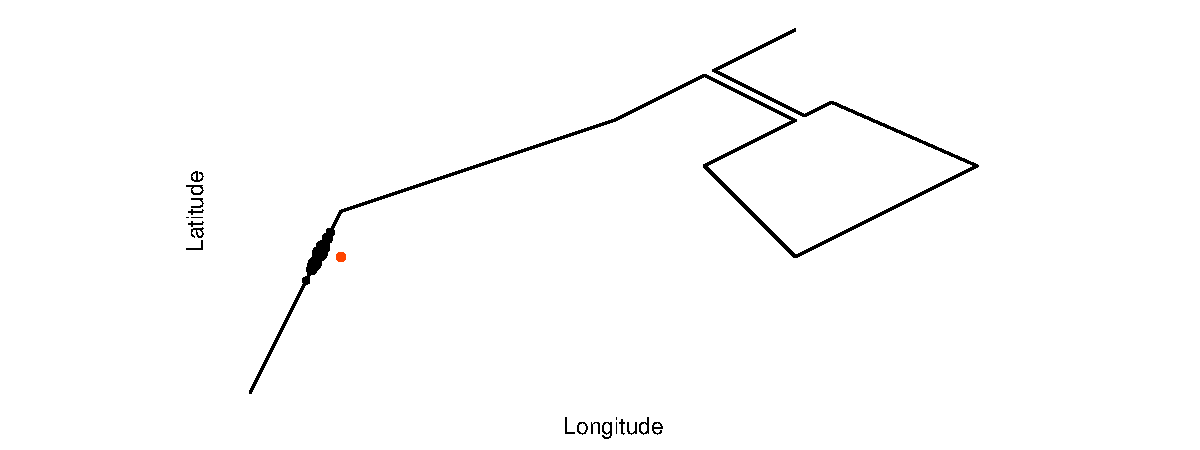
\includegraphics[width=\maxwidth]{figure/pf_wts-1} 

}

\caption[The \pf{} estimate of vehicle state after reweighting particles based on the likelihood, or distance from the observed location]{The \pf{} estimate of vehicle state after reweighting particles based on the likelihood, or distance from the observed location.}\label{fig:pf_wts}
\end{figure}


\end{knitrout}


\subsubsection{Trip updates}
\label{sec:lhood_trip}

As well as vehicle position updates from \GPS{} data, \GTFS{} provides trip updates from arrival and departure information. In many situations, it is difficult to infer a vehicle's trajectory based solely on \GPS{} data, and so trip updates are therefore an invaluable part of the update step. In this case, the \pf{} prediction step goes ahead as presented in \cref{sec:vehicle_model_trans}, but instead of then comparing the coordinates, the arrival or departure times are used to compute the liklelihood of the particles.


The trip update observations differ from the \GPS{} observations in that there are now three situations which can occur. The observation can be of an arrival time at stop $m$, $\Varr_m$, or it can be of a departure time, $\Vdep_m$. In the latter case, treatment of the observations depends on whether or not $\Varr_m$ was observed. This gives us three likelihood functions to derive,
\begin{itemize}
\item $p(\Varr_m | \Vstate_k)$, the arrival time likelihood function,
\item $p(\Vdep_m | \Vstate_k, \text{arrival missing})$, the departure time likelihood conditional
    on not having observed arrival time, and
\item $p(\Vdep_m | \Vstate_k, \text{arrival observed})$, the departure time likleihood conditional
    on having observed arrival time.
\end{itemize}


To compute the likelihood for these, we refer back to the dwell time model described in \cref{eq:stop_dwell_model,eq:stop_dwell_time}. Two additional parameters are also needed: the actual arrival time of the bus at stop $m$, $\Tarr_{m}$, and the measurement error of arrival time in seconds, $\TUerr$. The arrival time can be computed for each stop $m$ directly from the model (i.e., via interpolation). The departure time is then computed by summing the arrival and dwell times.


The observed arrival and departured times, denoted $\Varr_m$ and $\Vdep_m$, respectively, are assumed to each be normally distributed, with mean and variance determined by the described model. For arrival time, this is simply
\begin{equation}
\label{eq:tu_arr_lhood}
\Varr_m \sim \Normal{\Tarr_{mr}}{\TUerr}.
\end{equation}
and for departure time,
\begin{equation}
\label{eq:tu_dep_lhood}
\Vdep_m \sim \Normal{\Tarr_m + \pdwell_m}{\TUerr}
\end{equation}


In our \pf{} implementation, each observation will be processed individually; in situations where more than one type of observation is recieved, they are processed in chronological order and the particles reweighted between each. The necessary likelihood component for \cref{eq:vehicle_pf_reweight} is therefore
\begin{equation}
\label{eq:tu_obs_lhood}
p(\Vobs_k | \Vstate\vi_k) =
\begin{cases}
\frac{1}{\sqrt{2\pi\TUerr}}
    \exp\left\{
        -\frac{(\Varr_m - \Tarr_m)^2}{2\TUerr}
    \right\} & \text{for arrival times} \\
\frac{1}{\sqrt{2\pi\TUerr}}
    \exp\left\{
        -\frac{(\Vdep_m - \Tarr\vi_m - \pdwell\vi_m)^2}{2\TUerr}
    \right\} & \text{for departure times}
\end{cases}
\end{equation}
which allows the particle sample to be reweighted according to the temporal difference in arrival and departure times. This is demonstrated in \cref{fig:tu_update}.

\begin{knitrout}
\definecolor{shadecolor}{rgb}{0.969, 0.969, 0.969}\color{fgcolor}\begin{figure}

{\centering 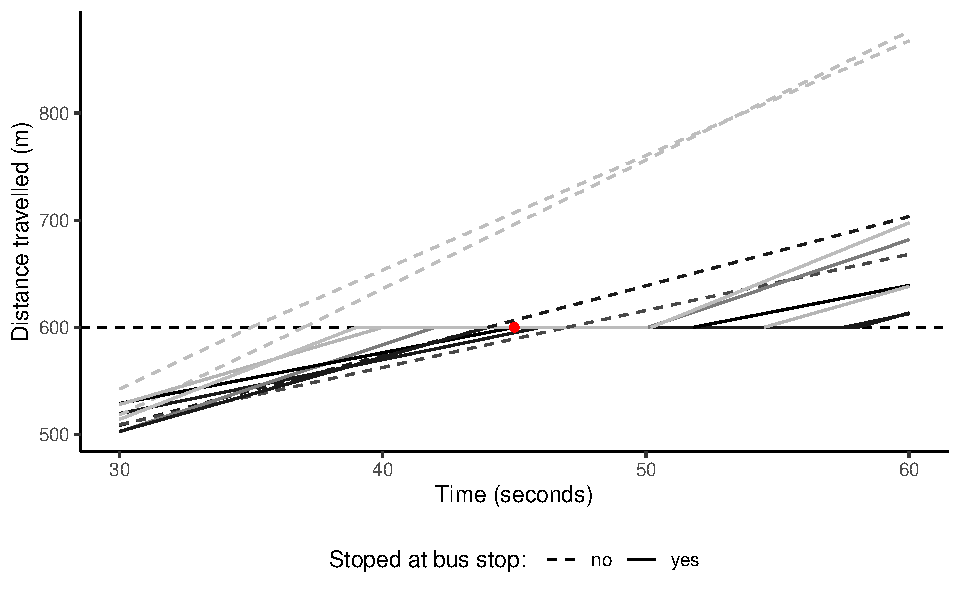
\includegraphics[width=0.8\textwidth]{figure/tu_update-1} 

}

\caption[Particle's travelling past an intermediate stop with an arrival time observation (red point)]{Particle's travelling past an intermediate stop with an arrival time observation (red point). Particle trajectories are coloured by whether or not they stopped. The likelihood is used to reweight the particles, indicated by line opacity.}\label{fig:tu_update}
\end{figure}


\end{knitrout}
